\documentclass[11pt,letterpaper]{article}


\usepackage[utf8]{inputenc}
\usepackage[spanish]{babel}
\usepackage{float}
\usepackage{xcolor}
\usepackage{verbatim}
\usepackage{mwe}
\usepackage{charter}
\usepackage{afterpage}
\usepackage{amsmath}
\usepackage{appendix}
\usepackage{ragged2e}
\usepackage{array}
\usepackage{etoolbox}
\usepackage{fancyhdr}
\usepackage{booktabs}
\usepackage{arydshln}
\usepackage[justification=justified,singlelinecheck=false,labelfont=bf,format=plain]{caption}
\usepackage[justification=justified,singlelinecheck=false,labelfont=bf,format=plain]{subcaption}
\usepackage{enumitem}
\usepackage[bottom=2.5cm,top=2.0cm,left=2.0cm,right=2.0cm]{geometry}
\usepackage{graphicx}
\usepackage{indentfirst}
\usepackage{mathtools}
\usepackage{multirow}
\usepackage{pdfpages}

\usepackage{subfiles}
\usepackage[compact]{titlesec}
\usepackage{blindtext}
\usepackage{stfloats}
\usepackage{lipsum} 
\usepackage{import}
\usepackage{pdfpages}
\usepackage{transparent}
\usepackage{xcolor}
\usepackage[colorlinks=true,linkcolor=blue]{hyperref}


\newcommand{\incfig}[2][1]{%
	    \def\svgwidth{#1\columnwidth}
	        \import{../img/}{#2.pdf_tex}
	}

	\pdfsuppresswarningpagegroup=1
\renewcommand{\familydefault}{\rmdefault}
\newcommand\blankpage{
    \null
    \thispagestyle{empty}
    \addtocounter{page}{0}
    \newpage}

\newcolumntype{L}[1]{>{\raggedright\let\newline\\arraybackslash\hspace{0pt}}m{#1}}
\newcolumntype{C}[1]{>{\centering\let\newline\\arraybackslash\hspace{0pt}}m{#1}}
\newcolumntype{R}[1]{>{\raggedleft\let\newline\\arraybackslash\hspace{0pt}}m{#1}}

    \setlist[itemize,1]{label=$\bullet$}
    \setlist[itemize,2]{label=$\circ$}
    \setlist[itemize,3]{label=$-$}
    \setlist{nosep}

\setlength{\columnsep}{30pt}

\titlelabel{\thetitle.\quad}

\pagestyle{fancy}
\fancyhf{}
      
\fancyfoot{}
\fancyfoot[C]{\thepage} % page
\renewcommand{\headrulewidth}{0mm} % headrule width
\renewcommand{\footrulewidth}{0mm} % footrule width

\makeatletter
\patchcmd{\headrule}{\hrule}{\color{black}\hrule}{}{} % headrule
\patchcmd{\footrule}{\hrule}{\color{black}\hrule}{}{} % footrule
\makeatother

\definecolor{blueM}{cmyk}{1.0,0.49,0.0,0.47}

%%%%%%%%%%%%%%%%%%%%%%%%%%%%%%%%%%%%%%%%%%%%%%%%%%%%%%%%%%%%%%%%%%%%%%%%%%%%%%%%%%%%%%%%%%%%%%%%%%%%%%%%%%%%%%%%%%%%%%%%%%%%%%%%%%%%%%%%%%%%%%%%%%%%%%%%%%%%%%%%%%%%%%%%%%%%%%%%%%%%%%%%%%%%%%%%%%%%%%%%%%%%%%
%%%%%%%%%%%%%%%%%%%%%%%%%%%%%%%%%%%%%%%%%%%%%%%%%%%%%%%%%%%%%%%%%%%%%%%%%%%%%%%%%%%%%%%%%%%%%%%%%%%%%%%
\title{RLC salida en R}    
\author{Álvaro Martín Romero}
\begin{document}
\maketitle
\tableofcontents
\section{Ejercicio 1}%
\label{sec:Muestra del circuito}
\subsection{Valor de la tensión de salida para la frecuencia de corte}
La tensión de salida para el circuito dado en salida de $R$ es:
\[
V_s=\frac{V_e R}{Ls+\frac{1}{Cs}+R}
.\] 
Hallamos la función de transferencia de este circuito utilizando su definición:
\[
    G\left( s \right) =\frac{V_s}{V_e} \implies G\left( s \right) =\frac{RCs}{\left( LCs^2+ RCs + 1 \right) }
.\] 
Haciendo $w_n=\frac{1}{\sqrt{LC} }$ y $RC=\frac{2\zeta}{w_n}$ con el cambio $s=j\omega$ el módulo de la función de transferencia es:
 \[
     G\left( j\omega \right) =\frac{2\zeta \frac{\omega}{\omega_n}}{\sqrt{\left( 1-\frac{\omega^2}{\omega_n^2} \right)^2+ \left( \frac{2\zeta \omega }{\omega_n} \right)^2  } }  
.\] 
Por tanto, si multiplicamos el módulo de la función de transferencia por la tensión de entrada y sustituimos los datos que nos da el problema $[R=220 \Omega ; L=10 mH; C=10nF; V_e =20Vpp=10 V]$:

\[
	\omega_{n}=\frac{1}{\sqrt{LC} }\implies f_n=\frac{1}{2\pi}\cdot \frac{1}{LC}=[L=10 mH; C= 10 nF]=15915.494 Hz 
.\] 
y 
 \[
	 \zeta=\frac{R}{2L}\sqrt{LC} =[R= 220 \Omega] =0.11
.\] 

Para $\omega=\omega_n= 15915.494Hz$ la tensión de salida calculada de forma teórica es:
\begin{equation}
	\boxed{ \mid V_s \mid =\frac{2\cdot 0.11}{2\cdot 0.11}=1 V}
\end{equation}

\subsection{Cálculo del ángulo de desfase}
El ángulo de desfase para el circuito RLC con salida en L se define como:
\begin{equation}
    \varphi=90^o - \arctan\left[ \frac{\frac{2\zeta \omega}{\omega_n}}{\left( 1-\frac{\omega^2}{\omega_n^2} \right) } \right] 
    \label{desfase}
\end{equation}
Donde para la frecuencia de corte: $\frac{\omega}{\omega_n}=1$, por tanto:

\begin{equation}
	\boxed{\varphi=0^o}
\end{equation}

\subsection{Tensión de salida una década por arriba y por debajo}
\begin{itemize}
	\item Para una década por encima:\\
\\
Esto es: 
\[
\frac{\omega}{\omega_n}=10
.\] 
Sustituyendo ese valor en la función de transferencia y despejando, nos queda que la tensión de salida es:
\begin{equation}
	\boxed{V_s=0.0222 V = 22.2 mV}
\end{equation}

\item Una década por debajo.\\
\\
Esto es :
\[
\frac{\omega}{\omega_n}=0.1
.\] 
Sustituyendo el valor en la función de transferencia y despejando nos queda que la tensión de salida es:
\begin{equation}
    \boxed{V_s=0.0222V = 22.2 mV}
\end{equation}
\end{itemize}
\subsection{Ángulo de desfase década por encima y debajo de la frecuencia de corte}
A continuación medimos el ángulo de desfase para una frecuencia igual a una década por arriba de la frecuencia de corte. \\
\\
Sustituyendo el valor de la frecuencia en \ref{desfase} vemos que el valor del ángulo de desfase es \[
    \varphi=90^o
.\] 
\subsection{Tensión máxima de salida y frecuencia a la que se encuentra}
Viendo el valor del módulo de la función de transferencia:
 \[
     G\left( j\omega \right) =\frac{2\zeta \frac{\omega}{\omega_n}}{\sqrt{\left( 1-\frac{\omega^2}{\omega_n^2} \right)^2+ \left( \frac{2\zeta \omega }{\omega_n} \right)^2  } }  
.\] 
Observamos que el valor máximo de la función de transferencia se obtendrá cuando el denominador sea mínimo. Esto se obtiene cuando $\omega=\omega_n$, es decir, cuando la frecuencia es la frecuencia de corte y, por tanto, la tensión máxima es la tensión hallada anteriormente; $V_{max}=1 V$

\section{Cálculo experimental en el simulador }
A continuación mostramos el circuito simulado en el programa MultisimLive con la frecuencia de corte que calculamos posteriormente:
\begin{figure}[H]
	\centering
	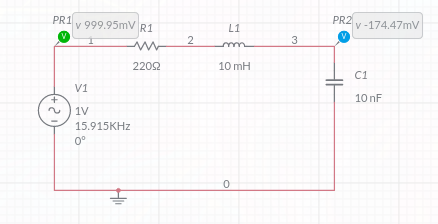
\includegraphics[width=0.6\textwidth]{../img/RLC_salida_R_circuito.png}
	\caption{Representación del circuito RLC con salida en R simulado en MultisimLive}
	\label{fig:img-RLC_salida_L-png}
\end{figure}
Para ver el valor de la tensión de salida en Multisim, simulamos el circuito para la gráfica 'Interactive', el resultado es el siguiente:
\begin{figure}[H]
	\centering
	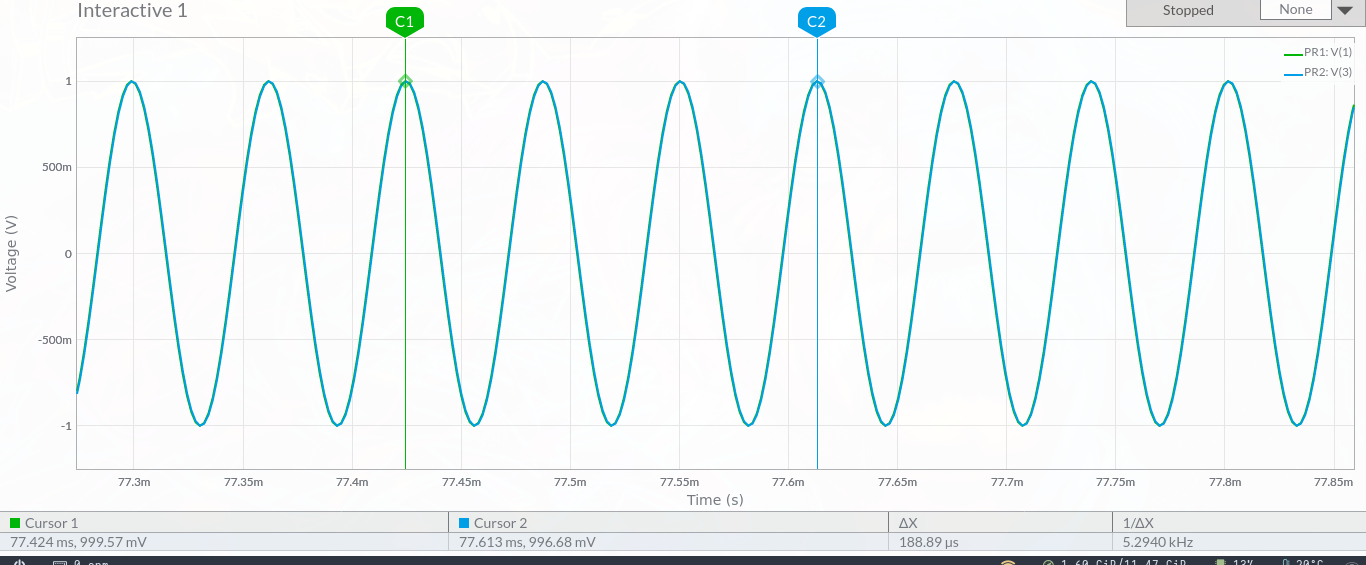
\includegraphics[width=0.8\textwidth]{../img/tension_fc_RLC_R.png}
	\caption{Representación del circuito en MultisimLive para observar la tensión de salida }
	\label{fig:}
\end{figure}
El cursor azul nos marca la tensión máxima de salida, esto es la misma que el cursor verde
\begin{figure}[H]
    \centering
    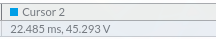
\includegraphics[width=0.4\textwidth]{../img/VmaxRLCR.png}
\end{figure}
\begin{equation}
	\boxed{V_s= 1 V}
\end{equation}
Esto es, la tensión de salida es igual a la tensión de entrada; o lo que es lo mismo, la función de transferencia es $1$, el resultado al que hemos llegado teóricamente
\subsection{Comprobación experimental en el simulador}
A continuación representamos el circuito en el diagrama de Bode para poder ver el desfase que hay para la frecuencia de corte $f_n=15915.494 Hz$. Esto lo hacemos con la función AC Sweep que tiene MultisimLive:
\begin{figure}[H]
	\centering
	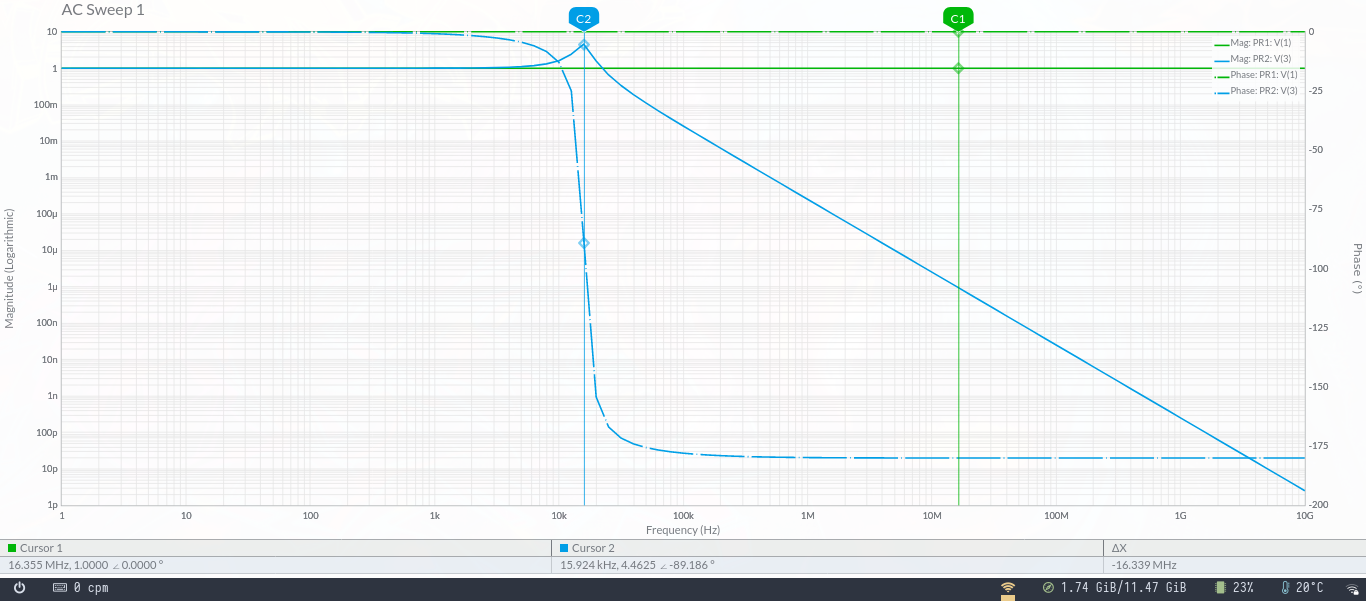
\includegraphics[width=0.8\textwidth]{../img/angulo_fc_RLC_R.png}
	\caption{Representación del diagrama de Bode del circuito para ver el desfase que se encuentra este en la frecuencia de corte}
	\label{fig:-img-angulo_fc-png}
\end{figure}
Como vemos en la gráfica, el ángulo de desfase lo podemos encontrar cuando la función de transferencia es 1, esto es, para la frecuencia de corte. El ángulo de desfase corresponde con el ángulo donde ocurre el pico de la gráfica vista en la figura anterior. Aproximadamente el valor del ángulo de desfase es:
\begin{equation} 
	\boxed{\varphi \approx 1^o}
\end{equation}
Este valor es aproximado debido a la sensibilidad del programa. Si pudiéramos encontrarnos en la frecuencia de corte exacta veríamos como el ángulo de desfase es $0$, tal como calculamos previamente.
\subsection{Simulación tensión salida década por arriba}
Simulamos el circuito una década por arriba:
\begin{figure}[H]
    \centering
    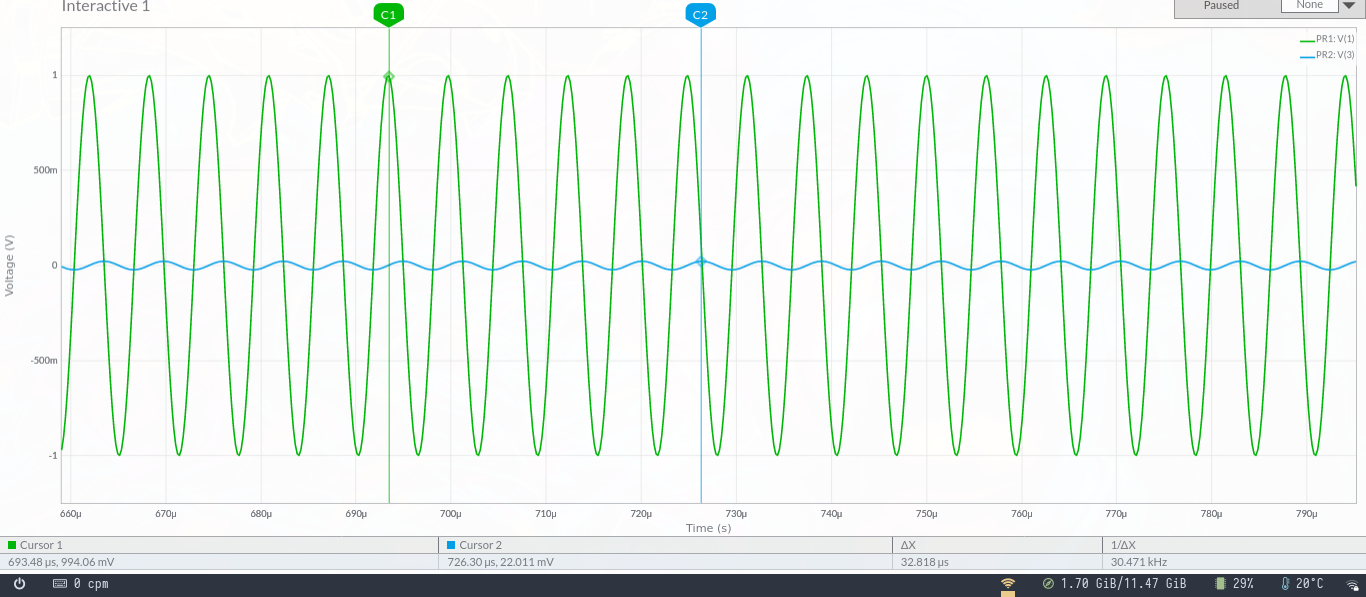
\includegraphics[width=0.8\textwidth]{../img/tension_darriba_RLC_R.png}
    \caption{Representación de la tensión de salida en el multisimLive para una década por encima}
    \label{fig:}
\end{figure}
Como vemos, el valor hallado experimentalmente para la tensión de salida (cursor azul0) es de \[
V=22.0 mV
.\] 
Un valor aproximadamente igual al hallado teóricamente.


\subsection{Simulación tensión de salida década por debajo}
Para una década por debajo, simulamos el circuito:
\begin{figure}[H]
    \centering
    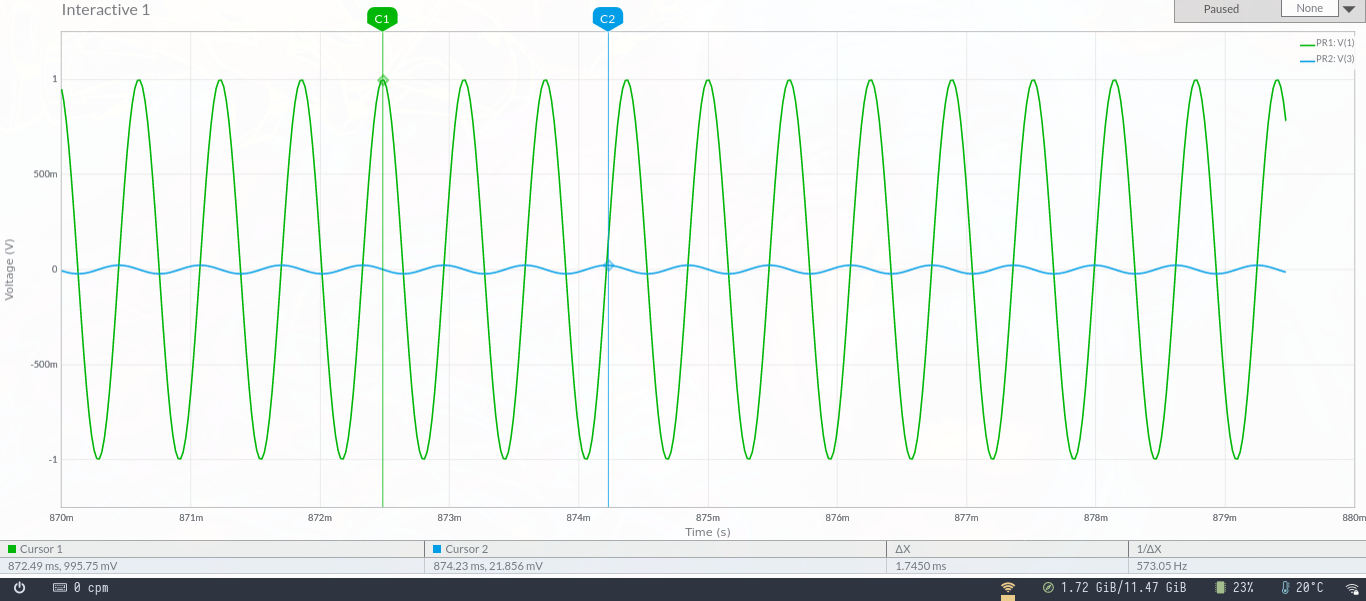
\includegraphics[width=0.8\textwidth]{../img/tension_dabajo_RLC_R.png}
    \caption{Representación del circuito en Multisim para una década por debajo de la frecuencia de corte}
    \label{fig:-}
\end{figure}    
Como vemos, el valor de la tensión de salida (cursor azul) corresponde a un valor de :
\[
V_s=0.022 V
.\] 
Esto es, un valor cercano a la tensión hallada teóricamente.

\end{document}

